% Dokumentinformationen
%Vorlage erstellt von Luca Mazzoleni aufbaudend auf der Vorlage von Stefan Reinli

% !TeX program = pdflatex
% !TeX encoding = utf8
% !TeX spellcheck = de_DE
% !BIB program = bibtex

\documentclass[
11pt,
final,
twoside,
a4paper]{article}
%%%%

% Document information
\newcommand*{\Title}            {Leistungselektronik-Entwickeln\\ für einen 1kW Windinverter Prototyp}
\newcommand*{\TitleInfo}        {Semesterarbeit HS 2018}
\newcommand*{\AuthorOne}		{Kris Wyss}
\newcommand*{\AuthorTwo}		{Stefan Bäbler}
\newcommand*{\Author}			{\AuthorOne, \AuthorTwo}
\newcommand*{\Prof}				{Prof. Dr. Jasmin Samjic}
\newcommand*{\Modul}			{Leistungselektronik}
\newcommand*{\Betreuer}			{Dr. Matthias Bucher, Thomas Franz}
\newcommand*{\Place}            {Rapperwswil}
\newcommand*{\LogoHSR}          {
\includegraphics[height = 1cm]{header/hsrlogo}}
\newcommand*{\LogoCompany}      {}      %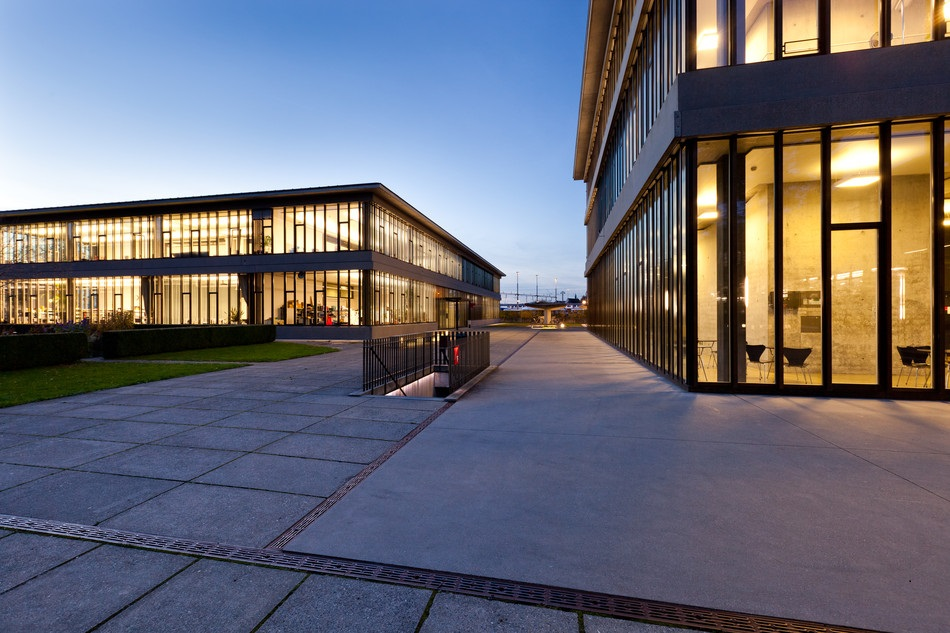
\includegraphics[height = 1cm]{header/logo}
\newcommand*{\Print}            {false} % true for black links (print version), false for color links (pdf version)

% Header
\usepackage[T1]{fontenc}	% ä,ü...
\usepackage[utf8]{inputenc} % utf-8 Unterstützung
\usepackage[ngerman]{babel} % Silbentrennung und Rechtschreibung Deutsch
\usepackage[{left=1.5cm,right=1.5cm,top=0cm,bottom=0cm}]{geometry} % Seitenränder Titelblatt


%%%%%%%%%%%%%%%%%%%%%%%
%% Packages
%%%%%%%%%%%%%%%%%%%%%%%
\usepackage[page,header]{appendix}
\usepackage{acronym} 		   % Für Abkürzungsverzeichnis
\usepackage{adjustbox} 		   % adjustbox, minipage..
\usepackage{amsmath}   		   % Allgemeine Matheumgebungen
\usepackage{amssymb}  		   % Fonts: msam,msbm, eufm & Mathesymbole, Mengen (lädt automatisch amsfonts)
\usepackage{array} 			   % Extending the array and tabular environment -> m,b,p,..
\usepackage{caption}  		   % Verändern der Schriftart von Bildunterschriften
\usepackage{changepage}
\usepackage{epstopdf}
\usepackage{expl3}
\usepackage{float}
\usepackage{framed, color}
\usepackage{fancyhdr}			%Für Kopf & Fusszeile
\usepackage{graphbox}
\usepackage{graphicx}
\usepackage{titletoc}			% Editieren des TOCs muss vor hyperref geladen werden
\usepackage{tocloft}			% Editieren des TOCs muss vor hyperref geladen werden
\usepackage{hyphenat}			%Wortumbruch
\hyphenation{he-lio-trope opos-sum}

\usepackage{listings}           % Erlaubt es Programmcode in der gewünschten Sprache zu hinterlegen (C++, Matlab,..)
\usepackage{longtable}
\usepackage{lastpage}			%Lastpage ref for Footer
\usepackage{marginnote} 		% Für Seitenkommentare \marginnote
\usepackage{mathtools}          % Vor mathabx laden!
\usepackage{mathabx} 			% Package mit vielen weiteren Mathe Symbolen
\usepackage{mparhack}  			% Improved marginpar placement
\usepackage{multicol} 			% In­ter­mix sin­gle and mul­ti­ple columns
\usepackage{multirow} 			% Create tabular cells spanning multiple rows
\usepackage{paralist}
\usepackage{pdfpages} 
\usepackage{pxfonts} 			% Mathsymbols
\usepackage[section]{placeins}  % Float-Barrier for Section
\usepackage{rotating} 			% Rotation tools, including rotated fullpage floats
\usepackage[onehalfspacing]{setspace}
\usepackage{scrhack}        	% Fixes koma-script incompatibilities
\usepackage{subcaption}
\usepackage{tabularx}
\usepackage{textcomp} 			% Wird für Copyright-Symbol,Währungen, Musikalische-Symbole benötigt
\usepackage[colorinlistoftodos,prependcaption,textsize=tiny]{todonotes}
\usepackage[most]{tcolorbox}
\usepackage{trfsigns}
\usepackage{varwidth}
\usepackage{wrapfig}
\usepackage{hyperref}
\usepackage{chngcntr}           %Nummerierung von Figuren Tabellen etc. Nach Kapitel
\usepackage{pdflscape}			%Eine Seite Landscape
%\usepackage{indentfirst}		%Einrücken von erster Zeile von Kapitel
	



%%%%%%%%%%%%%%%%%%%%%%%
%% PDF Meta Data
%%%%%%%%%%%%%%%%%%%%%%%

\hypersetup{
	pdfauthor={\Author},
	pdftitle={\Title},
	pdfsubject={\TitleInfo},
	%pdfkeywords={Some Keywords},
	pdfproducer={Latex with hyperref}
	%pdfcreator={pdflatex}
}
%\hypersetup{pdftex,
%	pdfauthor={\Author},
%	pdftitle={\Title},
%	pdfsubject={\TitleInfo},
%	%pdfkeywords={Some Keywords},
%	%pdfproducer={Latex with hyperref}
%	%pdfcreator={pdflatex}
%}

%%%%%%%%%%%%%%%%%%%%%%%
%% Setup Inkscape Import
%%%%%%%%%%%%%%%%%%%%%%%
\usepackage{import}
\graphicspath{{images/}}
\newcommand{\executeiffilenewer}[3]{%
	\ifnum\pdfstrcmp{\pdffilemoddate{#1}}%
	{\pdffilemoddate{#2}}>0%
	{\immediate\write18{#3}}\fi%
}
\newcommand{\includesvg}[1]{%
	\executeiffilenewer{#1.svg}{#1.pdf}%
	{inkscape -z -D --file=#1.svg %
		--export-pdf=#1.pdf --export-latex}%
	\input{#1.pdf_tex}%
}

%%%%%%%%%%%%%%%%%%%%%%%
%% Setup Tikz
%%%%%%%%%%%%%%%%%%%%%%%
\usepackage{tikz}
\usepackage{struktex}
\usepackage{schemabloc}
\usepackage[normalem]{ulem}
\usetikzlibrary{circuits}
\usetikzlibrary{arrows}
\usetikzlibrary{circuits.ee.IEC}
\usetikzlibrary{patterns}
\usetikzlibrary{positioning}
\usetikzlibrary{shapes,arrows}

\usetikzlibrary{patterns,decorations.pathreplacing}
\usetikzlibrary{decorations.pathreplacing}
\usetikzlibrary{external}
\usetikzlibrary{datavisualization}
\usepackage[europeanvoltages,
europeancurrents,
europeanresistors,   % rectangular shape
americaninductors,   % "4-bumbs" shape
europeanports,       % rectangular logic ports
siunitx,             % #1<#2>
emptydiodes,
noarrowmos,
straightvoltages,
smartlabels]         % lables are rotated in a smart way
{circuitikz}          %

\usepackage{pgfplots}
\usepackage{pgfplotstable}
\pgfplotsset{compat=newest}

\tikzstyle{block} = [draw, rectangle, minimum height=3em, minimum width=4em]
\tikzstyle{input} = [coordinate]
\tikzstyle{output} = [coordinate]
\tikzstyle{pinstyle} = [pin edge={to-,thin,black}]
\tikzstyle{sum} = [draw, circle, node distance=1em, minimum height=1.5em]
\tikzset{>=latex}
\tikzset{%
	block/.style    = {draw, thick, rectangle, minimum height = 3em,
		minimum width = 3em},
	sum/.style      = {draw, circle, node distance = 1.5cm}, % Adder
	input/.style    = {coordinate}, % Input
	output/.style   = {coordinate} % Output
}

\usepackage{pgfplots}
\pgfplotsset{width=10cm,compat=1.9}

\newcommand\Umbruch[2][3cm]{\begin{varwidth}{#1}\centering#2\end{varwidth}}


%%%%%%%%%%%%%%%%%%%%%%%
% Import Matlab Code 
%%%%%%%%%%%%%%%%%%%%%%%

\usepackage{listings}
\lstset{ 
    %basicstyle=\color{red},
breaklines=true,%
morekeywords={matlab2tikz},
keywordstyle=\color{blue},%
morekeywords=[2]{1}, keywordstyle=[2]{\color{black}},
identifierstyle=\color{black},%
stringstyle=\color{mylilas},
commentstyle=\color{mygreen},%
showstringspaces=false,%without this there will be a symbol in the places where there is a space
numbers=left,%
numberstyle={\tiny \color{black}},% size of the numbers
numbersep=9pt, % this defines how far the numbers are from the text
emph=[1]{for,end,break},emphstyle=[1]\color{red}, %some words to emphasise
%emph=[2]{word1,word2}, emphstyle=[2]{style},  
	frame=single,	                			% adds a frame around the code
%	tabsize=2,                				% sets default tabsize to 2 spaces
%	captionpos=b,                   			% sets the caption-position to bottom
}

%%%%%%%%%%%%%%%%%%%%%%%
% Caption Setup 
%%%%%%%%%%%%%%%%%%%%%%%
\captionsetup[figure]{labelfont={it,bf},textfont={it}}
\captionsetup[table]{labelfont={it,bf},textfont={it},singlelinecheck=off,justification=centering}
\captionsetup[lstlisting]{labelfont={it,bf},textfont={it}}
\captionsetup[subfigure]{labelfont=bf,textfont=normalfont,singlelinecheck=off,justification=centering}

\newenvironment{nscenter}
{\parskip=-5pt\par\nopagebreak\centering}
{\parskip=-15pt\par\noindent\ignorespacesafterend}

%Counting Anb. Tab, Fig
\counterwithin{figure}{section}
\counterwithin{table}{section}
\counterwithin{equation}{section}


%Rewritte Referenze Style and TOF,TOT
\renewcommand{\thefigure}{Abb. \arabic{section}.\arabic{figure}}
\renewcommand{\thetable}{Tab. \arabic{section}.\arabic{table}}
\renewcommand{\theequation}{\arabic{section}.\arabic{equation}}


\addto{\captionsngerman}{%
	%	\renewcommand*{\contentsname}{Inhalt}
	%	\renewcommand*{\listfigurename}{Abbildungen}
	%	\renewcommand*{\listtablename}{Tabellen}
	\renewcommand*{\figurename}{} %Delet Figure name 
	\renewcommand*{\tablename}{}
}
\setlength{\cftfignumwidth}{2cm}	% Width of equation number in List of Figure
\setlength{\cfttabnumwidth}{2cm}	% Width of equation number in List of Table

%List of Equations
\newcommand{\listequationsname}{Gleichungen}
\newlistof{myequations}{equ}{\listequationsname}
\newcommand{\myequations}[1]{% 
	\addcontentsline{equ}{myequations}{\protect\numberline{\theequation}#1}\par}
\setlength{\cftmyequationsnumwidth}{2cm}% Width of equation number in List of Equations


%%%%%%%%%%%%%%%%%%%%%%%%
%% Header and Footer %%
%%%%%%%%%%%%%%%%%%%%%%%%
\pagestyle{fancy} %eigener Seitenstil
\renewcommand{\sectionmark}[1]{\markright{#1}} %entfernt nummer vor section
\renewcommand{\subsectionmark}[1]{}
%twopage
%\ifthenelse{\isodd{\value{page}}}{\leftmark}{\rightmark}
% or with
%\fancyhead[OR]{} % "O" for "odd"
%\fancyhead[ER]{} % "E" for "even"

\fancypagestyle{plain}{
	\fancyhf{} %alle Kopf- und Fußzeilenfelder bereinigen
	
	\fancyhead[OR]{\textsl{\rightmark}}
	\fancyhead[ER]{\textsl{\rightmark}}
	\fancyhead[C]{} %zentrierte Kopfzeile
	\fancyhead[OL]{\Title}
	\fancyhead[EL]{\Title}
	\renewcommand{\headrulewidth}{0.4pt} %obere Trennlinie
	
	%\fancyfoot[OR]{Seite \thepage\ / \pageref{LastPage}}
	%\fancyfoot[ER]{\today}
    \fancyfoot[C]{\thepage}
   %\fancyfoot[EL]{Seite \thepage\ / \pageref{LastPage}}
	%\fancyfoot[OL]{\today}
	%\renewcommand{\footrulewidth}{0.4pt} %untere Trennlinie
}

\fancypagestyle{appendix}{
	\fancyhf{} %alle Kopf- und Fußzeilenfelder bereinigen
	\fancyhead[R]{} %Kopfzeile links
	\fancyhead[C]{} %zentrierte Kopfzeile
	\fancyhead[L]{} %Kopfzeile rechts
	\renewcommand{\headrulewidth}{0pt} %obere Trennlinie
	
	%\fancyfoot[OR]{Seite \thepage\ / \pageref{LastPage}}
	%\fancyfoot[ER]{\today}
	\fancyfoot[C]{\thepage}
	%\fancyfoot[EL]{Seite \thepage\ / \pageref{LastPage}}
	%\fancyfoot[OL]{\today}
	%\renewcommand{\footrulewidth}{0.4pt} %untere Trennlinie
}


\pagestyle{plain} %Pagesytle


%%%%%%%%%%%%%%%%%%%%%
%% Load HSR Color  %%
%%%%%%%%%%%%%%%%%%%%%
\usepackage{xcolor}
\usepackage{header/HSRColors}

%%%%%%%%%%
% Colors %
%%%%%%%%%%
\definecolor{black}{rgb}{0,0,0}
\definecolor{red}{rgb}{1,0,0}
\definecolor{white}{rgb}{1,1,1}
\definecolor{grey}{rgb}{0.8,0.8,0.8}
\definecolor{green}{rgb}{0,.8,0.05}
\definecolor{brown}{rgb}{0.603,0,0}
\definecolor{mymauve}{rgb}{0.58,0,0.82}
\definecolor{mygreen}{RGB}{28,172,0}
\definecolor{mygray}{rgb}{0.5,0.5,0.5}
\definecolor{mymauve}{rgb}{0.58,0,0.82}
\definecolor{mylilas}{RGB}{170,55,241}

\definecolor{gray80}{gray}{0.8}
\definecolor{gray60}{gray}{0.6}
\definecolor{gray40}{gray}{0.4}
\definecolor{gray20}{gray}{0.2}

%%%%%%%%%%%%%%%%%%%%%
%% Title %%
%%%%%%%%%%%%%%%%%%%%%



%Title Spacing-----------------------------------------
\usepackage{titlesec}
%\titlespacing{name=\section}{-\marginparwidth}{0pt}{0.2em}
%\titlespacing{name=\subsection}{-\marginparwidth+10pt}{0pt}{0.2em}
%\titlespacing{name=\subsubsection}{-\marginparwidth+14pt}{0.2em}{0.2em}
%\titlespacing{name=\paragraph}{-\marginparwidth+18pt}{0.2em}{0.2em}
%\newcommand{\subsectionbreak}{\clearpage}
%\setuphead[subsection][page=yes] % or page=right

%\titlespacing{name=\section}{1pt}{0pt}{0.2em}
%\titlespacing{name=\subsection}{1pt}{0pt}{0.2em}
%\titlespacing{name=\subsubsection}{1pt}{0.2em}{0.2em}
%\titlespacing{name=\paragraph}{1pt}{0.2em}{0.2em}

%%%%%%%%%%%%%%%%%%
%% Bibliography %%
%%%%%%%%%%%%%%%%%%
%\usepackage[fixlanguage]{babelbib}
%\selectbiblanguage{german}
\usepackage[backend=bibtex,style=ieee, defernumbers=false]{biblatex} %Do not use biber with TexWorks
\addbibresource{Literatur}


% Abbildungen im Quellenverzeichnis nach Alphabet ordnen, Rest nummerieren
%\DeclareFieldFormat{labelnumber}{\ifkeyword{abb}{\mknumalph{#1}}{#1}}


%%%%%%%%%%%%%%%%%%%%%%%%%%%%%%%%%%%
%% Itemize and Enumerate spacing %%
%%%%%%%%%%%%%%%%%%%%%%%%%%%%%%%%%%%
% \topsep: space between first item and preceding paragraph
% \partopsep: extra space added to \topsep when environment starts a new paragraph
% \itemsep: space between successive items. 
\usepackage{enumitem} % Controls Layout of itemize, enumerate, description
\setlist[itemize]{topsep=0pt,itemsep=-1ex,partopsep=1ex,parsep=1ex,after=\vskip0.1\baselineskip}
\setlist[enumerate]{topsep=0pt,itemsep=-1ex,partopsep=1ex,parsep=1ex,after=\vskip0.1\baselineskip}

%%%%%%%%%%%
%% Index %%
%%%%%%%%%%%
\usepackage{imakeidx}
\makeindex[intoc,columnseprule]
\indexsetup{firstpagestyle=plain}    % Show header/footer on index page

%-------------------------------------------------
% Marginalien/Seitenränder
%-------------------------------------------------
%\marginpar{Eine Randnotiz}
\newcommand{\marg}[1]{\marginpar{\raggedright \textbf{#1} }}	

%%%%%%%%%%%%%%%%%%%%%%%
%% Aligned footnotes %%
%%%%%%%%%%%%%%%%%%%%%%%
\usepackage[hang]{footmisc}
\setlength{\footnotemargin}{1em}

%%%%%%%%%%%%%
%% Tabular %%
%%%%%%%%%%%%%
\newcolumntype{L}[1]{>{\raggedright\arraybackslash}p{#1}} % Tabelleninhalt linksausgerichtet
\newcolumntype{R}[1]{>{\raggedleft\arraybackslash}p{#1}} % Tabelleninhalt rechtsausgerichtet
\newcolumntype{C}[1]{>{\centering\arraybackslash}p{#1}} %  Tabelleninhalt zentriert
\renewcommand\arraystretch{1.5}
\usepackage{array}
\usepackage{booktabs}

%%%%%%%%%%%%%%%%%%%%%%
%% Generelle Makros %%
%%%%%%%%%%%%%%%%%%%%%%

% If \Print=true, then make all links black for nicer print
\providecommand*{\True}{true}
\ifx \Print \True
\hypersetup{hidelinks, colorlinks, linkcolor = black, citecolor = black, filecolor = black, urlcolor = black}
\fi

%\parindent0pt % Zeileneinzug verhindern

%Matlab font
\newcommand{\matlab}[1]{\footnotesize{(Matlab: \texttt{#1})}\normalsize{}}

% Makro für Tabellenbilder gleich unterhalb der Linie
\newcommand\tabbild[2][]{%
	\raisebox{0pt}[\dimexpr\totalheight+\dp\strutbox\relax][\dp\strutbox]{%
		\includegraphics[#1]{#2}%
	}%
}

% Makro für Vorteile und Nachteil mit Plus und Minus
\newcommand\pro{\item[$+$]}
\newcommand\con{\item[$-$]}


%Float-Barrier for Subsection
\makeatletter
\AtBeginDocument{%
	\expandafter\renewcommand\expandafter\subsection\expandafter{%
		\expandafter\@fb@secFB\subsection
	}%
}
\makeatother


%%%%%%%%%%%%%%%%%%%%%%%%%%%%
% Mathematical Operators %
%%%%%%%%%%%%%%%%%%%%%%%%%%%%
\DeclareMathOperator{\sinc}{sinc}
\DeclareMathOperator{\sgn}{sgn}
\DeclareMathOperator{\Real}{Re}
\DeclareMathOperator{\Imag}{Im}
\DeclareMathOperator{\euler}{e}
\DeclareMathOperator{\cov}{cov}
\DeclareMathOperator{\PolyGrad}{PolyGrad}
\DeclareMathOperator{\gradient}{grad}
\DeclareMathOperator{\rotation}{rot}
\DeclareMathOperator{\divergenz}{div}
\DeclareMathOperator{\imag}{j}

%Grösse Integral anpassen
\def\Int{\mbox{\Large$\displaystyle\int$\normalsize}}
\def\Int{\mbox{\Large$\displaystyle\iint$\normalsize}}
\def\OInt{\mbox{\Large$\displaystyle\oint$\normalsize}}

%Makro für 'd' von Integral- und Differentialgleichungen 
\newcommand*{\diff}{\mathop{}\!\mathrm{d}}

%%%%%%%%%%%%%%%%%%%%%%%%%%%
% Fouriertransform %
%%%%%%%%%%%%%%%%%%%%%%%%%%%

\unitlength1cm
\newcommand{\FT}
{
	\begin{picture}(1,0.5)
	\put(0.2,0.1){\circle{0.14}}\put(0.27,0.1){\line(1,0){0.5}}\put(0.77,0.1){\circle*{0.14}}
	\end{picture}
}


\newcommand{\IFT}
{
	\begin{picture}(1,0.5)
	\put(0.2,0.1){\circle*{0.14}}\put(0.27,0.1){\line(1,0){0.45}}\put(0.77,0.1){\circle{0.14}}
	\end{picture}
}

%%%%%%%%%%%%%%%%
% Code Layout %
%https://en.wikibooks.org/wiki/LaTeX/Source_Code_Listings
%%%%%%%%%%%%%%%

%\definecolor{mygreen}{rgb}{0,0.6,0}
%\definecolor{mygray}{rgb}{0.5,0.5,0.5}
%\definecolor{mymauve}{rgb}{0.58,0,0.82}

\lstset{ %
    firstnumber=1,
    backgroundcolor=\color{white},   % choose the background color; you must add        \usepackage{color} or \usepackage{xcolor}
    basicstyle=\footnotesize\ttfamily, % the size of the fonts that are used for the code
    breakatwhitespace=false,         % sets if automatic breaks should only happen at whitespace
    breaklines=true,                 % sets automatic line breaking
    captionpos=b,                    % sets the caption-position to bottom
    commentstyle=\color{mygreen},    % comment style
    deletekeywords={...},            % if you want to delete keywords from the given language
    otherkeywords={...},             % if you want to add more keywords to the set
    escapeinside={\%*}{*\%},          % if you want to add LaTeX within your code
    extendedchars=true,              % lets you use non-ASCII characters; for 8-bits encodings only, does not work with UTF-8
    frame=single,	                 % adds a frame around the code
    keepspaces=true,                 % keeps spaces in text, useful for keeping indentation of code (possibly needs columns=flexible)
    keywordstyle=\color{blue},       % keyword style
    language=C++,                    % the language of the code   
    numbers=left,                    % where to put the line-numbers; possible values are (none, left, right)
    numbersep=5pt,                   % how far the line-numbers are from the code
    numberstyle=\tiny\color{mygray}, % the style that is used for the line-numbers
    rulecolor=\color{black},         % if not set, the frame-color may be changed on line-breaks within not-black text (e.g. comments (green here))
    showspaces=false,                % show spaces everywhere adding particular underscores; it overrides 'showstringspaces'
    showstringspaces=false,          % underline spaces within strings only
    showtabs=false,                  % show tabs within strings adding particular underscores
    stepnumber=2,                    % the step between two line-numbers. If it's 1, each line will be numbered
    stringstyle=\color{mymauve},     % string literal style
    tabsize=2,	                     % sets default tabsize to 2 spaces
    %title=\lstname                   % show the filename of files included with         \lstinputlisting; also try caption instead of title
}

\lstdefinestyle{customc++}{
    belowcaptionskip=1\baselineskip,
    %frame=L,
    xleftmargin=\parindent,
    language=C++,
    keywordstyle=\bfseries\color{blue},
    commentstyle=\itshape\color{mygreen},
    identifierstyle=\color{black},
    stringstyle=\color{gray},
}

\lstdefinestyle{cppunit}{
    belowcaptionskip=1\baselineskip,
    %frame=L,
    xleftmargin=\parindent,
    language=C++,
    keywordstyle=\bfseries\color{blue},
    keywordstyle=[2]\bf\color{black}, %not sure why \bf works, but it does
    commentstyle=\itshape\color{mygreen},
    identifierstyle=\color{black},
    stringstyle=\color{gray},
    keywords=[2]{  %Cpp Unit Keywords
        CPPUNIT_ASSERT,
        CPPUNIT_TEST,
        CPPUNIT_TEST_EXCEPTION,
        CPPUNIT_TEST_END,
        CPPUNIT_TEST_SUITE,
        CPPUNIT_TEST_SUITE_REGISTRATION,
        CPPUNIT_TEST_SUITE_END},
}

\lstdefinestyle{cppqt}{
    belowcaptionskip=1\baselineskip,
    %frame=L,
    xleftmargin=\parindent,
    language=C++,
    keywordstyle=\bfseries\color{blue},
    keywordstyle=[2]\bfseries\color{red},
    commentstyle=\itshape\color{mygreen},
    identifierstyle=\color{black},
    stringstyle=\color{gray},
    keywords=[2]{           % qt-Keywords
		Qt,
        SIGNAL,
        SLOT,
        QApplication,
        QDialog,
        QGridLayout,
        QPushButton,
        QLabel,
        QVBoxLayout,
        QHBoxLayout,
        QWidget,
        QGroupBox,
        QFont,
        QLineEdit,
        QRadioButton,
        QPen,
        QRect,
        QPaintEvent,
        QBrush,
        QPixmap,
        QPainter,
        QString,
        QPoint,
        update()},
}

\lstdefinestyle{cdoxy}{
    belowcaptionskip=1\baselineskip,
    %frame=L,
    xleftmargin=\parindent,
    language=C++,  
    keywordstyle=\bfseries\color{blue},
    commentstyle=\itshape\color{mygreen},
    identifierstyle=\color{black},
    stringstyle=\color{gray},
    otherkeywords={           % DoxygenKeywords
        ...,
        ....,
        @mainpage,
        @file,
        @author,
        @version,
        @date,
        @bug,
        @brief,
        @extended,
        @param,
        @return,
        @warning,
        @note,
        @see},
}

\lstdefinestyle{custommatlab}{
	belowcaptionskip=1\baselineskip,
	%frame=L,
	xleftmargin=\parindent,
	language=Matlab,
	basicstyle=\footnotesize\ttfamily,
	keywordstyle=\bfseries\color{blue},
	commentstyle=\itshape\color{mygreen},
	identifierstyle=\color{black},
	stringstyle=\color{mylilas},
}

%choose customstyle in DOC with \lstinputlisting[style=custom]{path}
\lstset{style=customc++}

\setcounter{secnumdepth}{4}

%\includeonly{sections/Einleitung,sections/Einleitung1,sections/Verzeichnisse}


% tcolorbox setup
\tcbset{width=(\linewidth-1mm)/2,before=,after=\hfill,arc=0mm,
	colframe=red!50!black,colback=white,colback = red!10}

\newcommand{\hsp}{\hspace{10pt}}
\titleformat{\section}[hang]{\Huge\bfseries}{\thesection\hsp\textcolor{gray80}{}\hsp}{0pt}{\Huge\bfseries}    %|
\titleformat{\subsection}[hang]{\huge\bfseries}{\thesubsection\hsp\textcolor{gray60}{}\hsp}{0pt}{\Large\bfseries} %|
\titleformat{\subsubsection}[hang]{\Large\bfseries}{\thesubsubsection\hsp\textcolor{gray40}{}\hsp}{0pt}{\large\bfseries} %|
\titleformat{\paragraph}[hang]{\large\bfseries}{\theparagraph\hsp\textcolor{gray20}{}\hsp}{0pt}{\large\bfseries} %|

% fontstyle
%\renewcommand\familydefault{\sfdefault}    % Arial

% Document=========================================
\begin{document}
    \pagenumbering{Roman}
    \thispagestyle{empty}
    \begin{titlepage}
	
	\begin{adjustwidth}{-25mm}{-45mm}
		%Seite einmitteln gemäss werten im geometry package:		
		\begin{adjustwidth}{35mm}{10mm}
		%	\textrm
			%{
				\textrm{	%sans serif schrift
				\vspace*{2cm}
				\begin{flushleft}
					\Huge \textbf{\Title}\\
					\vspace{.25cm}
					\Large \TitleInfo \\  %sffamily
				\end{flushleft}
			}
		\end{adjustwidth}
	
		\begin{figure}[ht]
			\centering
			\includegraphics[width = 0.9\textwidth]{images/Titelbild}
		\end{figure}
	
		\begin{figure}[ht]
			\centering
			\includegraphics[width = 0.3\textwidth]{images/IET_LogoGerman.pdf}
		\end{figure}

	
			\begin{adjustwidth}{35mm}{40mm}	
			\vfill
			\large
			\textrm{\textbf{Autoren}}\\
			\textrm{\Author} \\
			\textrm{\textbf{Dozent}}\\
			\textrm{\Prof}\\
			\textrm{\textbf{Betreuer}}\\
			\textrm{\Betreuer}\\
			\textrm{\textbf{Modul}}\\
			\textrm{\Modul}\\
			\hfill\hbox{}\\
			\textrm{HSR Hochschule für Technik Rapperswil}\\
			\hfill\hbox{}\\
			\textrm{\today}
            \vspace{1cm}
		\end{adjustwidth}	
	
	\end{adjustwidth}
\end{titlepage}

    \clearpage \pagebreak
    \thispagestyle{empty}
    \listoftodos
    \cleardoublepage \pagebreak
    \pagenumbering{arabic}
    \setcounter{page}{1}
    \thispagestyle{empty}

\newgeometry{left=2cm,right=4cm,top=1cm,bottom=1cm,headsep=1.5cm, marginparwidth=30mm,marginparsep=3mm,includeheadfoot}
\savegeometry{margin}
	\thispagestyle{empty}
	\section*{\huge Abstract}

\todo{Abstract muss geschrieben werden}

\newgeometry{left=2cm,right=2cm,top=1cm,bottom=1cm,headsep=1.5cm, marginparwidth=1mm,marginparsep=3mm,includeheadfoot} %Seitenränder Dokument ohne Titelblatt und Abstract
\savegeometry{no-margin}
	\begin{spacing}{1}
		\startcontents[sections]
		\printcontents[sections]{l}{1}{\setcounter{tocdepth}{4}\section*{Inhaltsverzeichnis}}	
	\end{spacing}
	\cleardoublepage 
	
%\loadgeometry{no margin}
	

%    \cleardoublepage
	\section{Einleitung}



 	\section{Pflichtenheft}

	 \vspace{-3cm}
\section{Projektplan}
%{\centering
%	\vspace{-0.4cm}}
%	\includegraphics[angle=90,clip, trim= 0.5cm 5.5cm 1cm 2cm, scale=0.83]{sections/Projektterminplan_SA.pdf}\par}

	\section{Entwicklung}
	\section{Redesign EMV-Filter}
\label{chapter_RedesignEMV}

Das Energieübertragungsnetz verträgt nur einen gewissen Prozentsatz an Strömen die einem ganzzahligen vielfachen des 50Hz Netzstromes entsprechen bevor es instabil wird. 
Deshalb wird in der Norm ???? der Grenzwert für den THDi (Total Harmonic Destroiten)
\begin{equation}
\text{THDi}=\dfrac{\sqrt{\sum\limits_\text{n=2}^{50} I^{2}_\text{n}}}{I_{1}}  \qquad\text{mit}\qquad \text{THDi} \leq \text{8\%}
\end{equation}
aufgeführt.
Zu beachten ist das die Zählvariable $n$ nur bis 50 geht.
Dies ist erstaunlich da höhere Harmonische noch einen beträchtlichen Einfluss auf den THDi haben bei einem PWM Signal das mit einer Frequenz von 10kHz generiert wird.
Diese Taktfrequenz erzeugt um 20kHz noch einige Harmonische, die beeinflussen den THDi. 
Dies ist in \ref{fig:THDiverg}, wo der THDi für $n=50$ und $n=300$ berechnet wurde, gut ersichtlich.
Wobei bei Zählvariable von 50 Harmonische bis 2kHz mit berücksichtigt werden und bei 600 bis 30kHz.
\begin{figure}[h!]
\begin{center}
	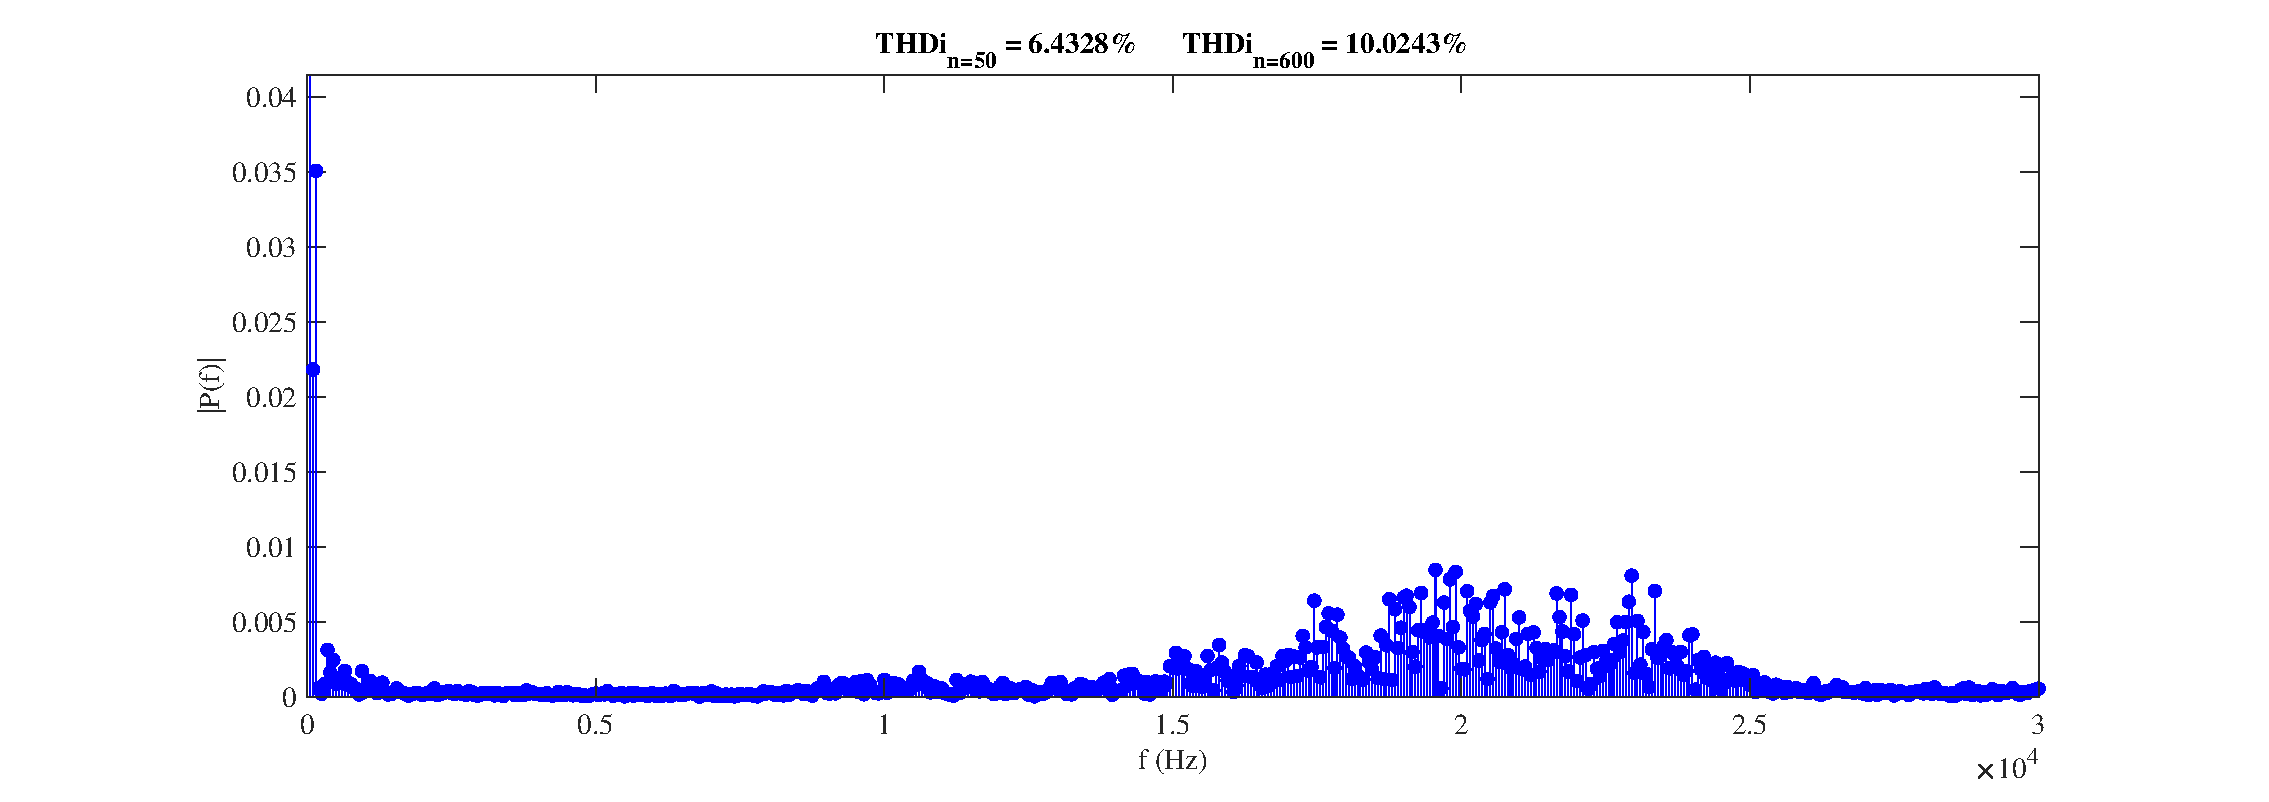
\includegraphics[width=\linewidth, height=0.25\textheight]{images/THDi_vergleich.eps}
	\caption{THDi Vergleich unterschiedliche Laufvariablen}
	\label{fig:THDiverg}
\end{center} 
\end{figure}

Der EMV-Filter (Elektromagnetische Verträglichkeit) hat primär zwei Ziele.

\begin{itemize}
	\item Filterung von Differential Mode Strömen
	\item Filterung von Common Mode Strömen
\end{itemize}

Die Filterwirkung ist bidirektional und schützt das Netz wie auch den Inverter vor denn hochfrequenten Strömen.
Schnelle Schaltvorgänge wie die PWM (Pulsweitenmodulation) begünstigen das entstehen von diesen. 

\subsection{Common Mode Ströme}
Wie die Namensgebung schon aussagt handelt es sich bei Common Mode Strömen um solche die auf 

\subsection{Differential Mode Ströme}
\label{chapter_diffModSt}

\subsection{Auslegung}
In diesem Kapitel ist beschrieben auf welchen technischen Grundlagen die im Inverter verbauten EMV-Filterkomponenten ausgelegt sind. 
Die klassischen Auslegungsmethoden (Bessel, Tschebyscheff, etc.) wie sie für Signalpfade gelehrt werden versagen leider bei einem EMV-Filter. 
Ein Grund dafür ist die Unbekannte Lastimpedanz vom Netz so wie die über die Last wechselnde Quellenimpedanz $Z_0$.
So wie auch die Idee der Filterauslegung, die darauf ab zielt die schlecht möglichste Impedanzanpassung, zwischen dem Inverter und Netz zu erzielen und gleichzeitig das System stabil so wie die Filterverluste möglichst gering zu halten.
Der Missmatch der Impedanzen sollte bei doppelter Schaltfrequenz maximal sein.
\subsubsection{Common Mode Filter}
Auf die Auslegung des Common Mode Filter wurde kein grosses Augenmerk gelegt, weil die parasitäre Kapazität
\begin{equation}
C_p=\dfrac{\epsilon \cdot A}{d}
\end{equation}
gegen Erde sehr gering ist. 
Dies weil kein elektrisch leitendes Gehäuse Vorhanden ist.
Der approximativ berechnete Widerstandswertwert 
\begin{equation}
X_c=\dfrac{1}{\omega \cdot C_p} \qquad\text{mit}\qquad
\omega = 2\cdot\pi\cdot f,
\end{equation}
bei Frequenzen um 20 kHz, liegt im einstelligen Mega $\Omega$ Bereich.
Somit wird der Common Mode Strom vernachlässig bar klein sein.

Um jedoch vorbereitet zu sein für ein späteres anbringen eines Gehäuses ist ein Commen mode choke im EMV-Filter verbaut. 
Es wurde die selbe gegen gewickelte Spule verwendet wie im Referenzmodel von TI ????.

\subsubsection{Differential Mode Filter}
Wie in \ref{chapter_diffModSt} beschrieben wird eine sehr starke Verzerrung des Stromes auf der Netzseite erwartet.
Diese Stromverzerrung weg vom Sinus generiert einen sehr hohen THDi.
Dieser gilt es zu minimieren bis die Normwerte eingehalten werden.
Es gibt zwei Möglichkeiten einen EMV Filter auszulegen. 
Erstere beruht auf Try\&error.  
Mit Hilfe einer Simulation und dem Austausch von den Filterkomponenten wird versucht eine günstige Komonenten Wahl zu finden. Dies kann erfolgreich sein aber bei falscher Komponenten Wahl auch zu einem instabilen Gesamtsystem führen.
Um dies zu umgehen gibt es diverse Step by Step Anleitung.
Mit solchen ist der EMV-Filter ausgelegt worden. 

\paragraph{Auslegung LC-Filter }
Als erstes wurde mit Hilfe von \cite{birichaEMC} ein LC-Filter ausgelegt.
Für die Auslegung von einem EMV-Filter bei Invertern ist es Wichtig den Gesamtwiderstand (Quellenwiderstand) 
\begin{equation}
Z_0=\frac{U_g^2}{P}
\end{equation}
des Inverters zu kennen, wobei die Netzspannung $U_g$ und die abgegeben Wirkleistung $P$ diesen beeinflussen.

Gemäss dem Middlebrock Stabilitätskriterium
muss für die Filterimpedanz $Z_f$ und den Quellenwiderstand $Z_0$ die Beziehung
\[
Z_f \ll Z_0
\]
gültig sein.
Wenn dies nicht gewährleistet ist kann das  Gesamtsystem instabil werden. Mit dieser Bedingung wird der Maximalwert
\begin{equation}
Z_{fmax} = \dfrac{1}{10}\cdot Z_0 \approx 5\Omega
\label{Zfmax}
\end{equation}
festgelegt.

Eine weitere Wichtige Eigenschaft ist die Eckfrequenz $f_c$ des EMV-Filters. Liegt sie zu nahe bei der Netzfrequenz $\omega_g$ oder ist sie zu hoch und liegt in der Nähe von der PWM Schaltfrequenz $\omega_s$ könnten sich Resonanzeffekte negativ auswirken. 

Somit gelten die Grenzbedingungen
\[
	Z_f < 5\Omega \qquad \text{und} \qquad 500Hz < f_c > 5kHz
\]
für die Auslegung.
 
Mit einem Impedanzdiagramm, welches als graphische Unterstützung dient, wird der Filter ausgelegt.
Ein solches ist in \ref{fig:ImpChart} dargestellt.

Zuerst wird $Z_{fmax}$ eingezeichnet (grün). 
Der ganze Bereich oberhalb von $Z_{fmax}$ (grau Hinterlegt) ist Sperrgebiet da eine Filterauslegung in diesem zu instabilem Gesamtsystem führen könnte. 
In einem zweiten Schritt wird die Grenzfrequenz $f_{Cmin}$ eingetragen.
Vom Schnittpunkt der zwei Geraden $Z_{fmax}$ und $f_{Cmin}$ werden zwei Linien im $45°$ Winkel gezeichnet. 
An diesen werden die Werte für $C_{fmin}$ und $L_{fmax}$ des LC-Filters abgelesen. 
Die Werte können im Erlaubten Bereich verändert werden dürfen aber die Grenzbedinungen nie verletzen.
Die grau gestrichelten Linien zeigen die Grenzen für die obere Grenzbedienung $f_{Cmax}$. 

Weil an Induktivitäten Ströme nicht springen können muss nun die grösstmögliche Induktiviät aus dem Diagramm herausgelesen werden.
Dann ist sicher das unter den gegebenen Grenzbedingungen die best mögliche Stromglättung realisiert wird.
Wie in \ref*{fig:ImpChart} ersichtlich sind dies einer Induktivität $L_{fmax} = 1.8mH$.
Daraus resultiert $C_{fmin} = 70 \mu F$.

Die Simulation hat gezeigt das eine L-Topologie nicht ausreicht um den THDi unter denn geforderten Normwert zu bringen.
In \ref{SimRes} wird näher auf die Resultate eingegangen.
\begin{figure}[h]
	\begin{center}
		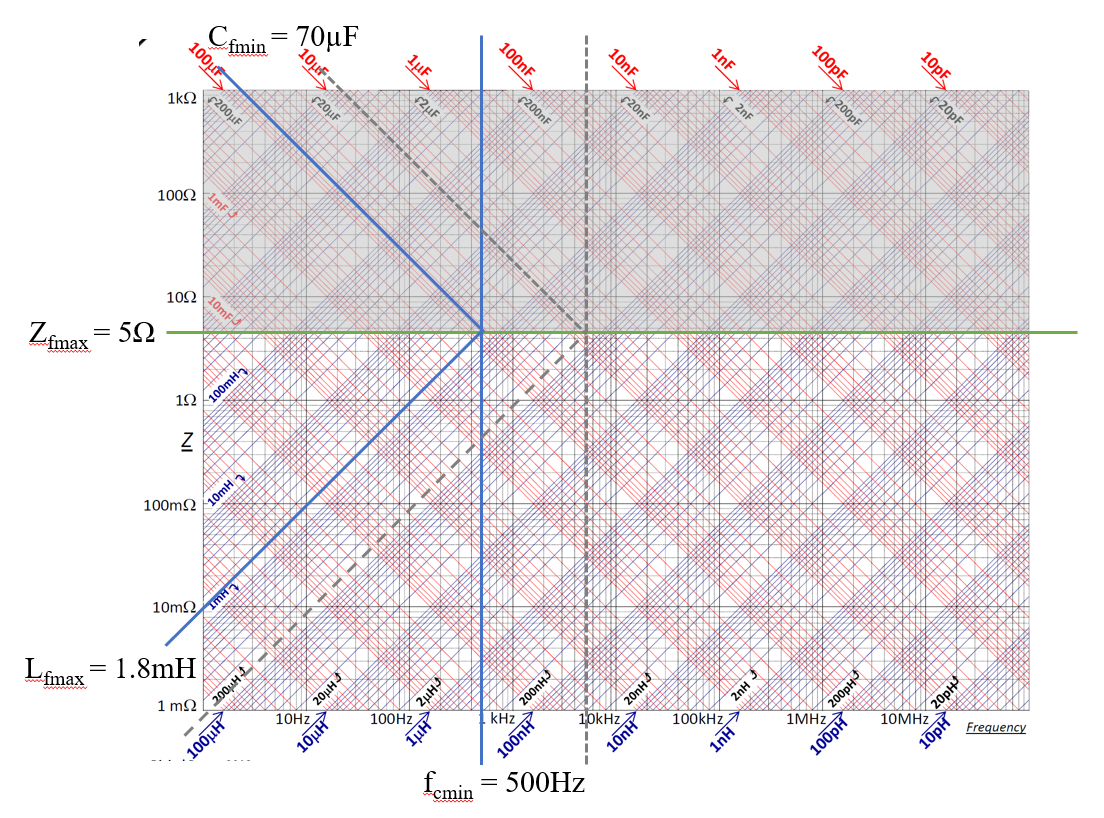
\includegraphics[width=\linewidth]{images/ImpChart}
		\caption{Impedanzdiagramm zur graphischen LC-Filter Auslegung}
		\label{fig:ImpChart}
	\end{center} 
\end{figure}

\paragraph{Auslegung LCL-Filter }
In einem zweiten Versuch ist ein Filter in $\pi$-Topologie entworfen worden. 
Die Auslegung des LCL-Filters, welche im folgenden beschrieben wird, beziehen sich auf die IEEE Publikation \cite{desLCLFilter}.

%SChema LCL Filter erstellen
Es gelten die selben Grenzbedingungen, für die maximale Filterimpedanz \ref{Zfmax} und für das Frequenzband der Grenzfrequenz, wie bei der Auslegung des LC-Filters um die Stabilität des Gesamtsystem zu gewährleisten.

Bei der Auslegung gibt es drei Freiheitsgrade mit denen das gewünschte Filter designet werden kann.
Als erstes wird festgelegt wie gross die inverterseitige Induktivität $L$ ist.
Diese Festlegung basiert auf dem Wissen das \ref{Zfmax} gelten muss.
Wir wählen 
\begin{equation}
L=\dfrac{1}{\omega_g\cdot X_L}\qquad \text{mit} \qquad   X_L=0.02\cdot Z_0
\end{equation}

In einem zweiten Schritt wird die Grösse der Filterkapazität $C_f$ festgelegt.
Diese soll maximal $5\%$ des kapazitiven Quellenwiderstandes 
\begin{equation}
C_0 = \dfrac{1}{\omega_g\cdot Z_0}
\end{equation}
sein.

Als letztes wird noch die Netzseitige Induktivität $L_g$ ausgelegt. 
Diese wird als Verältnissfaktor $r$ zwischen $L$ und $L_g$ 
angegeben.
In ???? ist ein Diagramm ersichtlich wo auf der Abszisse $r$ aufgetragen ist.
Es sind alle Grenzeinbedingungen ersichtlich welche eingehalten werden müssen.
Zsätzlich ist noch die minimale Dämpfung im Plot eingezeichnet. Diese wurde auch $0.2$ festgelegt was bedeutet das die Dämpfung der Oberwellen mindestens $80/$ ist.

\subsection{Simulationsresultate}
\label{SimRes}


% Notes:
%-Einfühung: Warum Filter? SChlechtmöglichste Abpassung an Netz um Oberwellen gehalt gemäss Norm einzuhalten. Commenmode und differenzialmode erklären -> kein augenmerk auf commenmode weil Kapazität nach erde so klein das keine Commenmode ströme fliessen können -> Berechnung auf Papier!
%
%
%- Netzimpedanz: Stand der Technik bei Hausinstallation ist max 1 Ohm Ohmscher Widerstand (Damit Schutzkonzept noch greift) Range ü[0.2; 1]
%Cosp min ist 0.92
%
%- Filter mit LCL und RL als last... Weil Filterperformace beim Geräteausgang gemessen wird. Deshalb L-Nezt kein gültiger Filterparameter.
%
%- Commenmode chock wie in Referenzmodel
%
%- Zwei Filterentwürfe
%1)  \cite{birichaEMC}.Ist entwurf für LC. Hat nicht gekalppt wegen Tradeoff zwischen Eckfrequenz/ZFilter zu ZQuelle/ -> Bild Impedanzchart einfügen!
%Und Bauteilwerte viel grösser! L=18mh C = 80uF
%
%2) Nach Paper: Ist Entwurf für LCL Filter... Step by Step
% Auslegung bei 12m/s?? Weil Z-b min! Um Stabilitätskriterium (Middlebrock) sicher nicht zu verletzen.
%	Schema Zeichnen, steps erklären, Maltap Plot Filterentwurf einfügen und erklären, 
%	Simulation bei 4m/s und 12m/s und die Viernetz parmamert (Nur R, Lklein und Rklein, Lkein und Rgross, Lgross und Rgross, Lgross und Rklein) -> in Simulationswerte für THD in Tabelle aufführen.
%    Tabelle mit Elememente aufführen.
%    
%
%
%\begin{center}
%  \begin{tabular}{|c|c|c|c|c|}
%  	
%  	\hline 
%  	V\textsubscript{wind} (m/s) & $L_{min}$/$R_{min}$ & $L_{min}$/$R_{max}$ & $L_{max}$/$R_{min}$ & $L_{max}$/$R_{max}$  \\ 
%  	\hline 
%  	12 &  &  &  &  \\ 
%  	\hline 
%  	7 &  &  &  &  \\ 
%  	\hline 
%  	4 &  &  &  &  \\ 
%  	\hline 
%  	
%  \end{tabular} 
%\end{center}
	\section{Hardware}

%Gate Driver: Selber wie bei Jonas2 da IGBT1 und IGBT3 genau anti parallel arbeiten -> Nur ein PWM für zwei IGBT notwendig...!
%Erster ausgewählter GAte Driver UCC27712 kann nicht verwendet werden da die PWM eingänge nicht galvanisch getrennt sind von den HI HL Ausgängen!!!
%
%Speisung +-15V um Tailingphenomen zu umgehen.
	\section{Schutzkonzept}

%Note Kris: Ein/Aus Schalter muss gegengekoppelte IGBT sein damit aus und eingeschalter werden kann. Sonst funktioniert der Kurzschlussschutz nicht beim ausschalten des Systems weil der einschalter erst beim nächsten Nulldurchgang sperrt, dann ist der KS-Triac bereits eingeschaltet und es entsteh ein Netzseitiger KS.

 
	\section{Resultat}
	\section{Zusammenfassung und Schlusswort}
	
%\loadgeometry{no-margin}
	\section{Erklärung zur Urheberschaft}
\vspace{0.8cm}
\textbf{Erklärung}\\

Wir erklären hiermit an Eides statt, dass ich die vorliegende Arbeit ohne Benutzung anderer als der angegebenen Hilfsmittel erstellt habe; die aus fremden Quellen direkt oder indirekt übernommenen Gedanken sind als solche kenntlich gemacht. Die Arbeit wurde bisher in gleicher oder ähnlicher Form keiner anderen Prüfungsbehörde vorgelegt und auch noch nicht veröffentlicht.\\
\vspace{0.8cm}\\

\begin{tabular}{l l}
    \textbf{Ort} & \textbf{Datum} \\
    \Place  & \today
\end{tabular}
\vspace{0.8cm}

\textbf{Unterschrift}\\
\vspace{0.2cm}
\AuthorOne \hspace{3cm} \AuthorTwo

\clearpage


	\section{Verzeichnisse}
%Abkürzungsverzeichniss, für schön ausrichten längste Abkürzung in eckige Klammer
\subsection{Abkürzungen}
\vspace{0.1cm}
\begin{acronym}[BA]
%\acro{Abkürzung}{Ausdruck ausgeschrieben}	
\acro{HSR}{Hochschule für Technik Rapperswil}
\acro{THDi}{Total Harmonic Distortion}
\acro{PWM}{Pulsweitenmoduliertes Signal}
\acro{EMV}{Elektromagnetische Verträglichkeit}
\end{acronym}	
\clearpage
\pagebreak


%Gleichungsverzeichnis
%\subsection{\listequationsname}
%\renewcommand*\listequationsname{}
%\listofmyequations\thispagestyle{fancy}
%\clearpage
%\pagebreak

%Abbildungsverzeichnis
\subsection{\listfigurename}
\renewcommand*\listfigurename{}
\listoffigures\thispagestyle{fancy}
\clearpage
\pagebreak

%Tabellenverzeichnis
\subsection{\listtablename}
\renewcommand*\listtablename{}
\listoftables\thispagestyle{fancy}
\clearpage
\pagebreak

%Quellenverzeichnis
\subsection{Quellenverzeichnis}
\printbibliography[heading=subbibliography,keyword=lit, title={Literaturquellen}]
\printbibliography[heading=subbibliography,keyword=manual, title={Datenblätter}]
\printbibliography[heading=subbibliography,keyword=online, title={Onlinequellen}]
\printbibliography[heading=subbibliography,keyword=abb, title={Bildquellen}]

\clearpage
	\pagestyle{appendix}
	\section*{Anhang}
\addcontentsline{toc}{section}{Anhang}
\appendix
\startcontents[sections]
\printcontents[sections]{l}{1}{\setcounter{tocdepth}{2}}
\clearpage
\pagebreak



\includepdf[pages={1},scale=0.95, pagecommand={\section{Anhangbsp mit PDF}},offset=0 -2cm]{sections/anhang/BA.pdf}
%
\includepdf[pages={2-},scale=0.95, pagecommand={\thispagestyle{appendix}}]{sections/anhang/BA.pdf}

\section{Anhang 2}
	\cleardoublepage
\end{document}
